
\newcommand{\imagw}[3]{
  \begin{figure}[!hbt]
    \centering
    \includegraphics[width=#1]{#2}
    \caption{#3}
    \label{fig:#2}
  \end{figure}
}

\newcommand{\imag}[2]{\imagw{16cm}{#1}{#2}}

\chapter{A prototype for spatio-angular illumination}
\label{sec:setup}
\begin{summary}
  We give a general overview of the system, followed by more detailed
  explanation of some if its components. Then we introduce a model
  that allows to construct optimized masks for spatio-angular
  illumination.
\end{summary}

\nomenclature{MEMI}{Micro-mirror enhanced micro-imaging. EU FP7
  project reference 215597.}
\section{Overview}
For the EU funded MEMI project it was decided to build a microscope
with two spatial light modulators as depicted in
\figref{fig:memi-simple}. The idea was to image one display (SLM2)
into the sample for spatial control. Work of other groups on
controlled light exposure microscopy (see section \ref{sec:CLEM}),
showed that it is possible to reduce unnecessary exposure of the
sample.

\begin{figure}[!hbt]
  \centering
  \def\svgscale{1.5}
  \input{memi-simple.eps_tex}
  \caption{Simplified schematic of the MEMI illumination system. A
    homogeneous spatially incoherent light source illuminates from the
    left. It is imaged by $L_1$ and $L_2$ into the intermediate image
    $F'$. Then the tubelens $L_3$ and the objective $L_4$ form an
    image of $F'$ in the sample plane $F$. The first spatial light
    modulator SLM1 is in the plane P', which is conjugate to the pupil
    (BFP) P of the objective. Using SLM1 we can control illumination
    angles in the sample. SLM2 is directly imaged into the sample and
    allows spatial illumination control.} \label{fig:memi-simple}
\end{figure}

An idea we haven't seen implemented so far, is to use another display
(SLM1) for angular illumination control. SLM1 is imaged into the back
focal plane of the objective. We hope to be able to reduce
out-of-focus exposure similar to the ultramicroscopy technique (see
section \ref{sec:light-sheet-microscopy}). However, our microscope
would work with sample in standard slides. We wouldn't need
sophisticated means of holding and rotating the specimen and our
technique could be more easily employed in automatic high-throughput
systems.

\begin{figure}[!hbt]
  \centering
  \def\svgscale{.43}
  \input{hourglass-all.eps_tex}
  \caption{{\bf (a)} Two fluorescent beads are illuminated by all
    angles that an objective can deliver. The sharp image of the
    in-focus bead is deteriorated by blurry fluorescence of the
    out-of-focus bead. {\bf (b)} Angular control allows selective
    illumination of the in-focus bead and results in a better image on
    the camera. {\bf (c)} Angular control is insufficient, when an
    extended in-focus area is illuminated. {\bf (d)} However,
    simultaneous spatial and angular control allows sequential
    excitation of the in-focus beads while excluding the out-of-focus
    bead.}
  \label{fig:hourglass-all}
\end{figure}

Unfortunately, the advantages of easy sample mount and reduced
phototoxicity come at a cost. The difficulty comes from the
illumination control itself. We have two displays that can project two
patterns with approximately $250\times 250$ pixels each. These are a
lot of degrees of freedom.  When we compare this situation to the
other techniques, we see: In ultramicroscopy no sample information is
required. Controlled light exposure microscopy the feedback loop takes
the local in-focus fluorophore concentration into account.

However, in a spatio-angular microscope, the feedback loop depends on
a lot more data, i.e.\ the full three-dimensional fluorophore
distribution in the specimen. Obviously, if this information was
known, there would be no need for imaging in the first place. Let us
assume, we know the exact sample, that we want to image. In reality,
we might only have an estimate of the sample.

In \figref{fig:hourglass-all} we visualize in a simple ray-based
model, how our optical system improves sample
illumination. Fortunately, it turns out that for the most useful
illumination strategies ray optics are sufficient. Nevertheless, some
design decisions require wave optics and we will discuss them on page
\pageref{sec:wave-constraints}.

\figref{fig:hourglass-all}~(a) depicts an illumination configuration,
that resembles the illumination in a confocal microscope. SLM1
transmits everything and the whole back focal plane of the objective
is illuminated. The illumination light is coming from the top.  The
pattern on SLM2 is a single bright spot and illuminates a fluorescent
bead in the focal plane. The incoming cone of light excites the
out-of-focus bead as well. The image on the right of the schematic
shows how an exposure of this scene would look on the camera of a
widefield microscope. The out-of-focus bead gives rise to blurry
background fluorescent light.

By changing the pattern on SLM1 we can limit the light rays, that
would excite the out-of-focus bead. This is indicated in
\figref{fig:hourglass-all}~(b). The camera would only show the image
of the in-focus bead and no background fluorescence from the
out-of-focus bead. Not exciting the out-of-focus bead has several
advantages:
\begin{description}
\item[Less phototoxicity:] Not exciting the out-of-focus areas is
  particularly useful for living biological specimen. Only with
  reduced phototoxicity long term time lapse experiments will show
  subtle biological effects. When imaging stacks the image quality of
  the spatio-angular microscope will surpass widefield microscopes add
  comparable overall dosage.
\item[Less noise:] There is less background light in the camera image,
  leading to a clearer image of the in-focus information. It would be
  possible to computationally distinguish and subtract out-of-focus
  light by structured illumination methods but these methods will not
  remove the Poisson distributed photon noise of the out-of-focus
  light.
\item[Precise light control:] In uncaging experiments, a compound is
  added to the medium, that breaks up or releases biologically active
  chemicals, when illuminated. In opto-genetics protein functions,
  e.g.\ an ion pump that can make a nerve cell fire \cite{Nagel2003},
  are controlled by illumination.

  Often a spatially resolved effect (e.g.\ activation of a single
  cell) is required. Until recently 2-photon excitation was the only
  option \citep{Pettit1997,Shoham2005} for such experiments. Only with
  the excitation point spread function of 2-photon microscopes, it is
  possible to limit the excited region to a confined volume with
  sufficiently small $z-$extent.

  Recently a holographic method was published that enables uncaging
  experiments with single-photon excitation \citep{Zahid2010}. It
  allows to sculpt the three-dimensional excitation volume and
  selectively activate groups of cells.

  Similarly our spatio-angular microscope could be
  used\footnote{Presently we have only implemented an optimization
    routine for a sphere model, this is probably not a good model to
    represent neurons.}, to selectively expose target neurons and
  prevent exposure of other cells. The holographic approach can
  achieve a higher light efficiency. However, the method for
  calculating the hologram is very different. In terms of current
  technology, their phase-only display is slower than our intensity
  modulators and potentially we could more easily provide a uniform
  illumination and prevent speckle.
\end{description}

The two schematics in \figref{fig:hourglass-all}~(a) and (b)
illuminate only one point in the focal plane. One could scan this
point over the whole sample. Then one could computationally
reconstruct a confocal image from the camera images but a tremendous
amount of data would have to be acquired. Therefore, it is useful to
simultaneously illuminate bigger regions in the sample.

However, if these regions are not carefully chosen, angular control
might not work any more. \figref{fig:hourglass-all}~(c) depicts a
sample with two in-focus beads and an out-of-focus bead in between. In
such a situation we would illuminate first one in-focus bead with an
appropriate pattern on SLM1 to prevent exposure of the out-of-focus
bead (\figref{fig:hourglass-all}~(d)) and then the other. 

One drawback of this technique is, that we require prior knowledge
about the fluorophore distribution in the sample, i.e.\ a three
dimensional model of what is going to be imaged.

In three-dimensional time lapse imaging of developing embryos a good
estimate is available when the stacks are acquired with high enough
temporal resolution. Opto-genetics experiments can be designed such,
that the three-dimensional distribution of neurons is known before
single neurons are triggered by light without exposing its neighbours.

For some sample types an estimation of the full three-dimensional
fluorophore concentration within the sample is not practical and might
be unnecessary. Instead, we believe we can project grating images with
the SLM2 and still vary the illumination direction with the mask on
the SLM1. The two camera images with structured illumination could then
be used to recover a sectioned image of the in-focus fluorophore
distribution \citep{2008Lim,Bozinovic2008,2009Santos}. Acquisition of
several such images with different MMA masks would allow to find the
angle with least out-of-focus contributions.


\subsubsection{Wave optical constraints in our spatio-angular microscope}
\label{sec:wave-constraints}
Earlier we claimed, that ray optics are sufficient to find good
patterns for SLM1 and SLM2. Now we will argue with wave optics and we
will see for which patterns the ray model will give wrong
results. Then we discuss the some design decisions in our
spatio-angular microscope.

By design all lenses in \figref{fig:memi-simple} are placed such, that
the back focal plane of one lens is the front focal plane of the
following lens. This simplifies the wave optical treatment of our
system. There is no need for free space propagation. We only have to
propagate the electric field from the front to the back focal plane
for each lens. This is done by a Fourier transform
\citep{Goodman1996}. At the objective $L_4$ we need to be careful. It
needs to be treated differently than standard thin lenses because of
its high aperture. The wave optical simulation is further complicated
by the need to sum over many coherent propagations to properly
represent spatially incoherent light source.  In
Appendix~\ref{sec:sim-angle} we show how to simulate the system using
Fourier optics.

For the current discussion we just note, that the electric fields in
the planes P' and F' in \figref{fig:memi-simple} form a Fourier
transform pair, i.e.\ the electric field illuminating SLM2 is the
Fourier transform of the field transmitted through SLM1. To discuss
this more thoroughly we distinguish the following configurations of
patterns on SLM1 and SLM2:
\newcommand{\sm}[1]{\raisebox{-2.5mm}{\includegraphics{slm-#1}}}
\begin{description}
\item[full SLM1 \sm{full}, point on SLM2 \sm{point}] This
  configuration corresponds to the confocal illumination in
  \figref{fig:hourglass-all}~(a). Angles from the full back focal
  plane will produce a spot in the sample with a size at the
  resolution limit of the objective.
\item[grating on SLM1 \sm{grating-circle}, point SLM2 \sm{point}] The
  grating on SLM1 gives rise to a diffraction pattern on SLM2. If the
  illumination was spatially coherent, there would be at least three
  spots, for $0^\textrm{th}$ and $\pm1^\textrm{st}$ orders. However,
  in our microscope the illumination is spatially incoherent, i.e.\
  each order would have an image of the light source attached to it.
  The small point on the SLM2 only transmits light from the
  $0^\textrm{th}$ order. Therefore, in the back focal would be
  illuminated uniformly and all information of the pattern on SLM1
  would be lost.
  
  For a grating on SLM1 with a big period, the images of the light
  sources overlap and the point on SLM2 would also transmit light from
  the first orders. However, the transmitted from the $+1^\textrm{st}$
  order light comes from a different area of the source than the
  transmitted light from the $-1^\textrm{st}$ order and they will not
  interfere to form an image of the grating in the back focal plane of
  the objective.

  This mode is not useful for illumination. The same intensity
  distribution in the sample can achieved more efficiently by a
  uniform pattern on SLM1.
\item[grating on SLM1 \sm{grating-circle}, full SLM2 \sm{full}]
  Displaying a grating on SLM1 will give rise to a diffraction pattern
  on SLM2. This will result in a bigger illuminated region in the
  sample. This configuration is also not useful and should be avoided.
\item[full SLM1 \sm{full}, grating on SLM2 \sm{grating}] The grating
  on SLM2 will produce a diffraction pattern in the back focal plane
  of the objective with an image of SLM1 attached to each order. Like
  this: \sm{3bigger}. For a very fine grating, the first orders can be
  far apart and only few of the rays can form an image (see also
  Appendix \ref{sec:apotome}).
\item[partial SLM1 \sm{half}, grating on SLM2\sm{grating}] To ensure a
  high contrast of the grating in the sample, it is useful to limit
  the angular range of angles using the pattern on SLM1, so that the
  first orders completely fit\footnote{For a high contrast of a very
    fine grating within the sample the described illumination scheme
    alone is not sufficient. The polarization has to be turned
    according to the grating orientation has well. This could be added
    to our prototype, however it currently not implemented.} through
  the back focal plane of the objective: \sm{3big}.
\item[full SLM1 \sm{full}, full SLM2 \sm{full}] This configuration
  corresponds to a standard widefield microscope. This and similar
  patterns with big convex illuminated areas can be represented with
  good accuracy by a model based on ray optics.
\end{description}

\subsubsection{Discussion of wave optical effects}
From the comparison we see, that our configuration with the second SLM
in the intermediate image F' (\figref{fig:memi-simple}) doesn't allow
high frequency patterns on SLM1. High frequency components of the
image of SLM1 in the back focal plane are heavily influenced by the
pattern on SLM2.

This configuration, which places more importance on SLM2 is a
deliberate design decision.  We chose configuration because we think
it is more important to have high resolution control of the spatial
light distribution in sample space.

One can estimate that with a $63\!\!\times\!\!/1.4$ objective it is
sufficient to illuminate a window with 1\% of the back focal plane
diameter, in order to illuminate an area with $\unit[3]{\mu m}$ in the
sample.  Therefore, as long as the patterns on both SLMs are
sufficiently simple, i.e.\ cover more than a few percent of the full
area, are simply connected and convex, %FIXME simply connected?
the ray-based model is a good representation of the system.

Projecting fine gratings into the sample using SLM2 is possible, but
higher diffraction orders fill more of the back focal plane. Therefore
grating projection will limit the usefulness of angular illumination
control.

The electric fields after SLM1 and on SLM2 form a Fourier transform
pair. Heisenberg's uncertainty relation prevents illumination of a
small spot on SLM2 when SLM1 only transmits very little. It is known,
that a Gaussian transmission function on SLM1 would achieve the
smallest possible spot on SLM1. Therefore, we decided to use a spatial
light modulator, that can display gray values.

\section{Detailed explanation of the optical components}

As opposed to the schematic in the previous system, our spatial light
modulators are reflective.  Also, both displays are not direct
intensity modulators.  \figref{fig:memi-real} shows a schematic of the
light path in the combined angular and spatial control system.

A laser light source is scrambled by a rotating micro-lens array and
mixed in an integrating tunnel with a quadratic cross section.

The distance between the exit of the integration tunnel and the lens
$L_1$ is equal to the focal distance of $L_1$. The MMA is positioned
in the other focal plane of $L_1$. The micro mirror array
\citep{Berndt2007,Schmidt2010,Berndt2010} consists of $256\times 256$
mirrors with a pitch of \unit[16]{$\mu$m} (see \figref{fig:mma} and
\figref{fig:mma-closeup}). Each mirror hangs on two thin hinges and
can be tilted by up to $2^\circ$ by electrostatic fields. This
corresponds to out-of-plane deflections of $\pm\unit[250]{nm}$.  CMOS
circuits below each mirror allow to maintain a constant tilt for
hundreds of milliseconds. A dedicated control board can set new
analogue voltages for each mirror in \unit[850]{$\mu$s}. An accuracy
of $\lambda/100$ for the precision of the actuation is reported
\citep{Berndt2011}. Therefore, the MMA is a programmable phase mask of
high efficiency and can achieve frame rates of up to \unit[1]{kHz} at
duty cycles up to \unit[50]{\%}. In a Fourier filtered configuration
it can display gray value images without the need for
time-multiplexing.  An On/Off-contrast from 300 to 800 in the
wavelength range from the UV upto NIR can be achieved
\citep{Berndt2011}.

When all mirrors of the MMA are flat, an image of the tunnel exit $F'''$
is formed in the plane of the aperture $B_1$. The size of the aperture
is chosen to transmit just this image. When mirrors of the MMA are
tilted, they will slightly deflect the light, so that it no longer
passes through the aperture $B_1$. $B_1$ acts as a Fourier filter (or
Schlieren optical system).

If the mirrors of half of the device are deflected to fulfil the blaze
conditions\footnote{This is limited by the maximum tilt angle and
  possible for wavelengths up to \unit[1000]{nm}} then the mirrors will
send all the light into the first order and nothing through the
aperture $B_1$.  The region in the image in $P'$ corresponding to the
tilted mirror will be dark.

The lenses $L_2$ and $L_3$ relay the image of the tunnel exit $F'''$
from $F''$ into the plane $F'$ with the LCoS (ForthDD SXGA, pixel
pitch $\unit[13.62]{\mu m}$) \citep{Cartwright2007}. The polarizing
beam splitter ($45^\circ$ wire grid polarizing beam splitter, Moxtek,
UT, US) reflects linearly polarized light towards the LCoS\footnote{In
  order to prevent spurious reflections at the PBS back surface
  (without wire grid coating) and to improve contrast, the incoming
  light should already be polarized}. The electric field vibrates
perpendicular to the paper plane. Depending on the LCoS pixel state
(on or off) an LCoS pixel can rotate the polarization of the returning
light. Light that is polarized in the paper plane is
transmitted\footnote{As it is used in transmission a curvature of the
  PBS doesn't affect the quality of the LCoS image in the sample $F$
  as if the PBS was used in reflection.}  into the illumination tube
lens $\textrm{TL}_\textrm{ill}$ by the PBS (see \figref{fig:lcos} for
a photograph showing tube lens, PBS and LCoS). In order to project a
very fine grating into the sample, the grating lines must be parallel
to the paper plane.

The LCoS is ferroelectric \citetext{\citealp[see][]{1991Saleh} and
  \citealp[p.~192]{Goodman1996}}.  Its liquid crystals can be driven
very fast between two bi-stable orientations. In order to prevent a
net current, which would eventually destroy the device, its driver
always displays an inverted image after the wanted one. Therefore it
is necessary to modulate the light source accordingly.


\begin{figure}[H]
  \centering
  \def\svgscale{2}
  \input{memi-real.eps_tex}
  \caption{Schematic of the light path through our microscope. Laser
    light enters from the lower left, is scrambled and homogenized to
    illuminate the full MMA and LCoS. $F$ is the field plane in the
    sample and its primed versions are conjugated planes. $P$ is the
    pupil of the objective. $B_0$ and $B_1$ are adjustable circular
    apertures. PBS is a polarizing beam splitter. DBS is a dichroitic
    beam splitter.}
  \label{fig:memi-real}
\end{figure}


The lenses $L_3$ and $\textrm{TL}_\textrm{ill}$ relay the Fourier
filtered MMA image from $P'$ into the pupil $P$ of the objective. In
order to accommodate objectives with various back focal plane
diameters, the illumination tube lens is built out of three lens
groups. Its focal length can be varied from \unit[222.8]{mm} up to
\unit[445.4]{mm} (see \figref{fig:memi-sketch} for a drawing with the
focal length of the other lenses). The lens groups of
$\textrm{TL}_\textrm{ill}$ move such, that the image of the LCoS
behind $\textrm{TL}_\textrm{ill}$ stays in infinity and the MMA
(plane $P''$) is imaged into the pupil $P$, which is \unit[250]{mm}
behind the tube lens. Only the lens groups within the tube lens
move, everything else in the system is
fixed. \figref{fig:tubelens-bfp} shows the pupil plane $P$ for two
different settings of the focal length of the tube lens.

Fluorescence light returns from the objective and is reflected by the
dichroitic beam splitter (DBS) through the detection tube lens
$\textrm{TL}_\textrm{det}$ and is imaged on the camera. Note that the
detection works with full efficiency.

\begin{figure}
   \centering
   \def\svgscale{2}
   \input{memi-sketch.eps_tex}
   \caption{Schematic of the lenses in the MEMI system and their focal
     lengths. The focal length $f_\textrm{TL}$ of the tube lens can be
     varied. This allows to scale the second intermediate image
     $r''_\textrm{MMA}$ of the micro mirror array to fit the back
     focal plane of different objectives. Dimensions in mm.}
   \label{fig:memi-sketch}
 \end{figure}
 

\imagw{14cm}{setup-photo-blueprint}{The wide field epi-fluorescent
  microscope with attached illumination head. The positions of the two
  spatial light modulators (Micro mirror array (MMA) and liquid
  crystal on silicon display (LCoS)) are indicated. Drawing by Josef
  Wenisch (In-Vision, Austria).}

\imagw{14cm}{mma}{{\bf left:} Scanning electron microscope image of
  the micro-mirror array (MMA).  The pixel pitch of the device is
  \unit[0.016]{mm}. The hinges for the tilt movement and the
  electrodes are clearly visible. {\bf middle:} Optical reflective
  microscope image of the MMA. {\bf right:} exaggerated rendering of
  how a 8x8 checker board pattern would be displayed on the
  device. Electron and optical micrograph by Fraunhofer IPMS Dresden
  (Germany)}

\begin{figure}[!hbt]
  \centering
  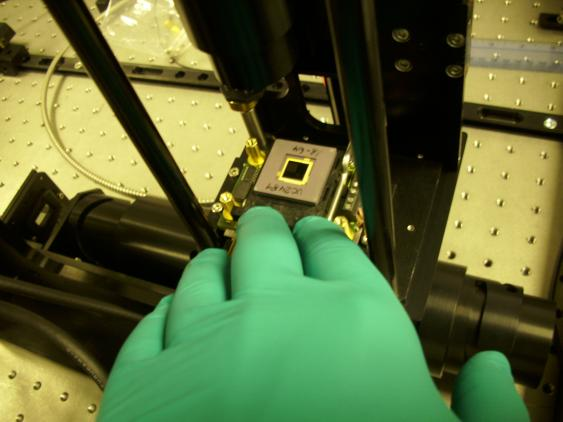
\includegraphics[width=7cm]{mma-plain}
  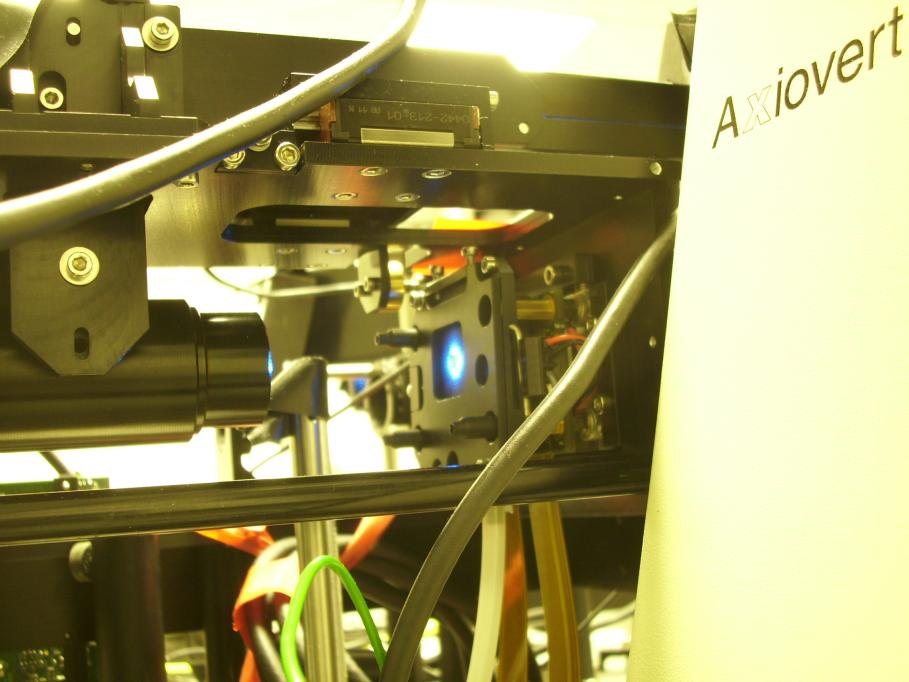
\includegraphics[width=7cm]{mma-ill}
  \caption{{\bf left:} Micro mirror array chip during installation of
    the optics. {\bf right:}~Illuminated micro mirror array in the
    aligned system.}
  \label{fig:mma-closeup}
\end{figure}

\begin{figure}[!hbt]
  \centering
  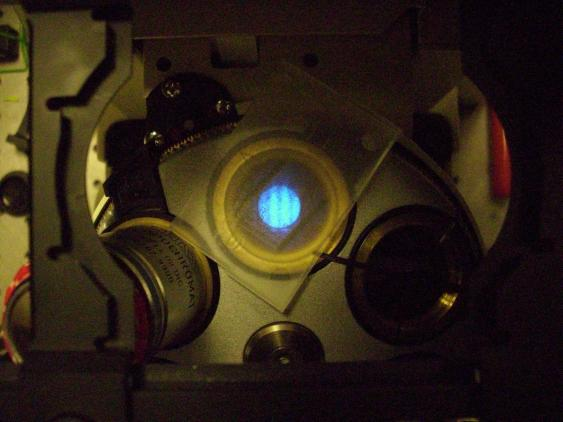
\includegraphics[width=7cm]{bfp1}
  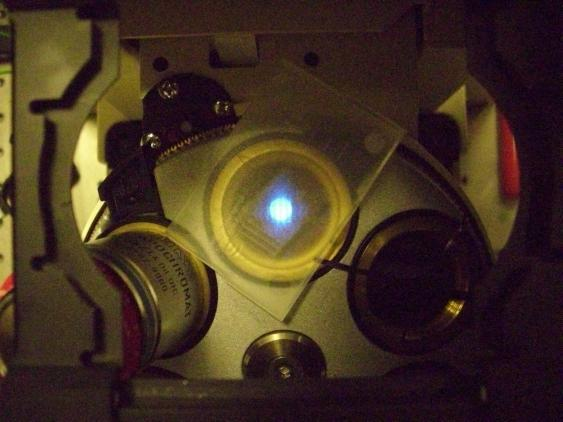
\includegraphics[width=7cm]{bfp2}
  \caption{Images of the micro mirror array in the back focal plane
    with different settings of the variable tube lens. The micro mirror
    array displays the same image (a disk) in both cases.}
  \label{fig:tubelens-bfp}
\end{figure}

\imagw{5cm}{lcos}{The black cylinder on the left is the variable tube
  lens. Behind this is the polarizing beam splitter and the
  ferroelectric liquid crystal on silicon display.}
\newpage
\section{Electronics for synchronization}
Both spatial light modulators can run at most with $50\%$ duty
cycle. Therefore it is necessary to synchronize the displays. Their
controllers allow to upload several hundred frames of image data
before an experiment and keep them in local storage. Images can then
be selected by fast function calls over USB (LCoS) or Ethernet (MMA).

The camera (Clara, Andor PLC, Belfast, Northern Ireland) as the
slowest device is chosen as the master. The camera provides two TTL
outputs. The output ``fire'' is high while the camera is
integrating. The output ``shutter'' goes high \unit[1]{ms} before
``fire'' and provides enough time (\unit[$>850$]{$\mu$s}) for the MMA
controller to tilt and let the mirrors settle.

The LCoS controller can only be programmed to a limited number of
discrete image times (\unit[20]{ms}, \unit[10]{ms}, \unit[5]{ms},
\unit[200]{$\mu$s}) and it is not straight forward to change this via
USB interface. Therefore we always work with a fixed integration time
of \unit[20]{ms}. The ``fire'' output of the camera also switches the
laser on using an acousto-optic modulator (AOM).

When the z-stage is used, the camera is stopped until the stage has
reached its target position.

\begin{figure}[!hbt]
  \centering
  \input{memi-electronics.eps_tex}
  \caption{The camera triggers both spatial light modulators with its
    TTL outputs. The acousto-optic modulator sends light into the
    system during camera integration.}
  \label{fig:memi-electronics}
\end{figure}

\section{Alignment of the displays}

In order to be able to predict which position on the camera will be
illuminated by a particular pixel of the LCoS a calibration procedure
is run. For this a fluorescent plane is selected as a specimen. Then
single spots are scanned for a grid of $10\times10$ positions over the
LCoS. The resulting spots on the camera are located and four
parameters defining the rigid transform between camera and LCoS are
estimated (scale, rotation angle, translation in x and y, see
Appendix~\ref{sec:rigid}).

Using these parameters one can then convert between camera and LCoS
coordinates (see \figref{fig:screen_lcos-calib}). Changing the focal
length of the illumination tube lens or a change on the camera position
generally requires a new calibration.

\imagw{7cm}{screen_lcos-calib}{{\bf left:} Mask that is displayed on
  the LCoS. {\bf right:} Camera image of fluorescent plane illuminated
  by mask. The orange lines indicate the borders of the original
  pattern.}

The MMA is aligned by displaying an annular ring on the MMA and
matching it to the ring of a phase objective.


\section{Ray-based illumination optimization}
In order to make use of the spatio-angular illumination system it is
necessary to produce masks for the two spatial light modulators, that
will reduce unnecessary illumination in the sample.

\subsection{Index matched sphere model}
\label{sec:shadow-map}
One useful simple model are spheres. They can model fluorescent beads
or nuclei in a \emph{C.~elegans} embryo. \figref{fig:render} displays
a model of a \emph{C.~elegans} embryo, constructed from
three-dimensional data of a confocal microscope. The nuclei are
relatively sparse. In order to illuminate one or a few nuclei we might
be able to find a path for the excitation light that doesn't intersect
out-of-focus nuclei -- or at least avoids them. In our spatio-angular
microscope the illumination pattern is represented by two masks. One
for the LCoS and another one for the MMA. In the following we will
construct an algorithm to find such optimized illumination
patterns. For example the red rectangle (with $\sim\unit[4]{\mu m}$ on
the side) would be selected for illumination with the LCoS. The red
cylinder indicates the angle that would be least obscured by
out-of-focus nuclei.

\imagw{6cm}{render}{Rendering of a sphere model, fitted to one time
  frame of a three-dimensional confocal video of a developing
  \emph{C. elegans} embryo (strain AZ212, data provided by Jean-Yves
  Tinevez (Institut Pasteur, Paris) by finding local maxima in the
  difference of Gaussian filtered data \citep{Santella2010}.}

\subsection{Tracing in illumination direction}
\imagw{12cm}{scan-mosaic_testsample_n100_3_7_5_big_label}{Test case
  for spatio-angular illumination. A target sphere is moved out of a
  layer of spheres. {\bf (a-c)} Rays from the back focal plane are
  traced through the target sphere and the total intersection length
  with out-of-focus spheres is plotted in the diagrams.}

First we assume the beads are embedded in index matched medium. Then
rays only refract at the Gaussian sphere of the objective lens and it
is insignificant how far the target bead is from the interface between
coverslip and medium. Other lenses, such as $\textrm{TL}_\textrm{ill}$
are assumed to be perfect lenses and are not considered here.

Initially we investigated a very simple optimization routine (see
\figref{fig:scan-mosaic_testsample_n100_3_7_5_big_label}). A circular
window with radius $r$ is placed into the back focal plane. Rays from
the centre and periphery of the window are traced through the target
and into out-of-focus spheres. The intersection length of each ray
with each sphere is summed and plotted into a diagram.

\figref{fig:scan-mosaic_testsample_n100_3_7_5_big_label}~a) depicts
the collected values for a point-like window.
\figref{fig:scan-mosaic_testsample_n100_3_7_5_big_label}~b) shows the
same for a window with a diameter of 5\% of the back focal plane. The
left column in the table below the images lists the minimal values
over the full back focal plane. For small windows, a few of the rays
can hit the target without intersecting any other spheres. Increasing
the window size blurs the features in the diagrams.

Here we would choose the window with $r=0.15$
(\figref{fig:scan-mosaic_testsample_n100_3_7_5_big_label}~c)). It
still has a low minimum but the largest amount of light would reach
the target. If we chose a too small value for $r$ we would on the one
hand send only a very small amount of light into the specimen. On the
other hand the field distribution in $P$ is related to the Fourier
transform of the field distribution in $F$ and due to Heisenberg
uncertainty relation a small $r$ in $P$ would illuminate the full
field in $F$.

If we chose a bigger value for $r$ many rays would intersect with
out-of-focus objects.
 
\imagw{12cm}{scan-mosaic_nuc12_n100_3_7_5_big_label}{Raytrace for
  circular window optimization in illumination direction. A window
  with 33\% BFP diameter would be used to illuminate the target
  nucleus.}

\figref{fig:scan-mosaic_nuc12_n100_3_7_5_big_label} shows a similar
raytrace for a sphere model of a \emph{C.~elegans} embryo and chooses
a window size and position which in this sense is optimal.

With the MMA we have a very versatile display and we don't
have to limit ourselves to circular windows. Also the raytraced
optimizations can look noisy when not enough rays are sent through the
sample.
\subsection{Tracing in detection direction}
\label{sec:trace-detect}
For this reason we decided to trace rays from out-of-focus nuclei
through the target into the back focal plane.

\figref{fig:img2-montage_hor}~C) depicts the results of tracing
through a single target point and the out-of-focus spheres in B) in
illumination direction. Note how each out-of-focus spheres result in a
deformed blob in the back focal plane. 

It should be quite clear that the image in
\figref{fig:img2-montage_hor}~D) displays nearly the same information
but was obtained with much less computation.  Here 16 rays were trace
(see Appendix~\ref{sec:sphere-projection}) from the periphery of each
out-of-focus nucleus and one from the centre and the resulting
triangle fan was rasterized into the image. We call this image a
shadow map.


In order for our spatio-angular system to work, neither the MMA, nor
the LCoS should display masks with only a few white pixels. Ray based
simulations are not good models in this case (see
Appendix~\ref{sec:sim-angle} for a description of a wave optical
treatment) and illumination light would simply be impractically low.

For this reason the trace of \figref{fig:img2-montage_hor}~D) is
insufficient. Instead of one target point a sufficiently big area in
the model should be sampled. We sum each of the corresponding shadow
maps into a new one (see the two images on the left in
\figref{fig:bfp2-bfp-images-and-model}. Then we threshold the
accumulated shadow map, so that only the angles with least
out-of-focus targets are illuminated. Finally we blur the mask with a
Gaussian filter in order to prevent ringing of the light distribution
(Gibbs' phenomenon) in sample space.
%FIXME heisst das so?

The diagram on the right of \figref{fig:bfp2-bfp-images-and-model}
displays a sphere model of three-dimensionally distributed beads
($\unit[2]{\mu m}$ diameter, yellow-green, in oil). We obtained this
model with our microscope by displaying several gratings on the LCoS
at full angular illumination and doing a structured illumination
reconstruction (in each pixel the maximum of each pattern minus minimum
of each pattern) of sectioned slices. A matching difference of
Gaussian filter and local maximum search in the three-dimensional
volume gives the centres of the beads.

After constructing the model, the microscope continuously moves the
z-stage onto each bead and illuminates them with their optimized
illumination angles. Bead~26 has been illuminated with very high
angles in order to prevent exposure of the bunch of beads further away
from the objective. Bead~5 is far from any other beads and therefore
more angles can be used for its illumination.


\imagw{14cm}{img2-montage_hor}{{\bf A)} Schematic of the rays between
  back focal plane and sample. {\bf B)} Out-of-focus spheres and the
  target point define a double cone of rays that should not be
  illuminated. {\bf C)} Tracing rays in illumination direction from
  the back focal plane through the sample is an expensive operation
  and results in unnecessarily exact results. {\bf D)} Tracing in
  detection direction from the periphery of out-of-focus spheres
  through a target point into the back focal plane gives nearly
  identical results (shadow map) and is more computationally
  efficient.}

% some raw data with beads in dvi system:
% /mnt/backup/backups-london/mnt/floh/sda3/martin/0226/winterseminar/0216_6
\imagw{10cm}{bfp2-bfp-images-and-model}{{\bf right:} Sphere model of a
  sample with three-dimensionally distributed beads. {\bf left:}
  Optimized MMA masks to illuminate bead 26 or bead 5. The red circles
  indicate the periphery of the BFP of the objective.}



%\imagw{12cm}{structured}{Images of a $\unit[3]{\mu m}$ bead within
%  slightly fluorescent embedding medium under different illumination
%  conditions using a $63\times/1.38$ objective.}




\subsection{Coping with index mismatch of the embedding medium}
So far the described algorithms assumed ideal samples which have been
embedded in a medium with a refractive index, the objective was
designed for.

Biological samples are often embedded in water. However, it might
still be useful, to image with an oil objective. Then the additional
refraction at the glass--water interface has to be taken into account
for spatio-angular illumination.

This makes the task of predicting where to mask the MMA in order to
protect out-of-focus beads more complicated. To circumvent the
spherical aberrations, we have to limit the range of angles, that are
simultaneously illuminating and shift the illumination spot on the
LCoS to correct for the transversal focus shift ($q$ in
\figref{fig:aberration-sketch} right). For this we must have a good
estimate of the distance of the sample from the coverslip--water
interface. See Appendix~\ref{sec:raytrace} for a description of the
raytrace algorithm.

Using an oil immersion objective has the following advantage: By
sending the illumination rays into the sample at a steep angle, close
to the TIRF angle, we can generate a thin sheet of light (see
\figref{fig:hilo}).


\begin{figure}[!hbt]
  \centering
  \def\svgscale{.3}
  \input{screen_0_lines.eps_tex}\qquad
  \input{aberration-sketch.eps_tex}
  \caption{{\bf left:} Rays are starting from periphery of
    out-of-focus nucleus, hitting the target and refracted at the
    water--coverslip interface. {\bf right:} Due to spherical
    aberrations, rays from an on-axis point are shifted to $q(r)$ on
    the camera (where $r$ relates to the angle of the ray in the
    sample). }
  \label{fig:aberration-sketch}
\end{figure}

\begin{figure}[!hbt]
  \centering
  \def\svgscale{.3}
  \input{shift-correction.eps_tex}
  \caption{{\bf top:} A straight ray illuminates a bead embedded in
    oil. {\bf middle:} Embedding the sample in water results in
    refraction of the ray. {\bf bottom:} The refraction can be
    compensated by shifting the target area on the LCoS.}
  \label{fig:shift-correction}
\end{figure}
 
% our reports: they were often corrected by Susan, so i should have a look
% MEMI_WP6_D6_5_Report.pdf     angular clem with grating on lcos
% 6.7    drawing of setup, alignment, sync image, only 11 of the 24 bitplanes
% 6.8a   full field angular control with mma (i used too large images on lcos)
%        rendering of c. elegans embryo, psf calc, ray model,
%        first (yellow) raytraces
% 8.6a   sync image with 11 out of 24
